\documentclass[a4paper,12pt]{article}
\usepackage{cmap}
\usepackage[T2A]{fontenc}
\usepackage[utf8]{inputenc}
\usepackage[russian]{babel}
\usepackage{indentfirst}
\usepackage{graphicx}

\usepackage{geometry}
\geometry{left=3cm}
\geometry{right=2cm}
\geometry{top=2cm}
\geometry{bottom=2cm}

\usepackage[hidelinks]{hyperref}

\usepackage{titletoc}
\newlength{\seclenght}
\settowidth{\seclenght}{6. }
\dottedcontents{section}[\the\seclenght]{}{\the\seclenght}{2mm}
\newlength{\subseclenght}
\settowidth{\subseclenght}{6.2. }
\dottedcontents{subsection}[\the\subseclenght]{}{\the\subseclenght}{2mm}
\newlength{\subsubseclenght}
\settowidth{\subsubseclenght}{6.2.8. }
\dottedcontents{subsubsection}[\the\subsubseclenght]{}{\the\subsubseclenght}{2mm}
\newlength{\pagereflenght}
\settowidth{\pagereflenght}{\pageref{LastPage}}
\contentsmargin{\the\pagereflenght}
\renewcommand{\thesection}{\arabic{section}.}
\renewcommand{\thesubsection}{\thesection\arabic{subsection}.}
\renewcommand{\thesubsubsection}{\thesubsection\arabic{subsubsection}.}
\setcounter{tocdepth}{3}

\usepackage{enumitem}
\usepackage{longtable}
\usepackage{tabu}
\usepackage{lastpage}

\begin{document}
\begin{titlepage}
\begin{center}
\hrule\vspace{1em}
\bf Московский государственный технический университет им. Н.Э.\,Баумана\\
Кафедра <<Системы обработки информации и управления>>\\[1em]
\hrule
\end{center}

\vfill

\noindent УТВЕРЖДАЮ:\\[1em]
\underline{\hspace{12em}} Галкин~В.\,А.\\[1em]
<<\underline{\hspace{1em}}>> \underline{\hspace{6.5em}} 2017~г.

\vfill\vfill

\begin{center}
\large Программа и методика испытаний\\
к~курсовой работе\\
{\Large<<Локальная безадаптерная сеть>>}\\
(вариант №\,26а)\\
по~курсу {\Large<<Сетевые технологии в~АСОИУ>>}
\end{center}

\vfill\vfill\vfill

\begin{tabular*}{\textwidth}{l@{\extracolsep{\fill}}l}
&ИСПОЛНИТЕЛИ:\\[1em]
&\underline{\hspace{12em}} Лещев А.\,О., ИУ5-64\\[1em]
&\underline{\hspace{12em}} Мельников К.\,И., ИУ5-64\\[1em]
&<<\underline{\hspace{1em}}>> \underline{\hspace{6.5em}} 2017~г.\\
\end{tabular*}
 
\vfill

\begin{center}
Москва~--- 2017~г.\\[1em]
\hrule
\end{center}

\end{titlepage}

\setcounter{page}{2}
%\tableofcontents
%\clearpage

\section{Наименование}
Локальная безадаптерная сеть.

\section{Назначение разработки}
Программа должна реализовывать функцию передачи файлов по~локальной сети с~возможностью докачки после восстановления прерванной связи, состоящей из~двух персональных компьютеров, соединённых через интерфейс RS-232C нуль-модемным кабелем.

\section{Последовательность испытаний}
Все пункты методики испытаний следует выполнить последовательно.

\section{Методика испытаний}
Далее $A$~--- пользователь передающей программы, $B$~--- пользователь принимающей программы.
\begin{center}
\begin{longtabu} to \linewidth {|l|X|X[2]|X[2]|}
\hline
\textbf{№}	&	\textbf{Проверяемая функция}	&	\textbf{Действия пользователя}	&	\textbf{Результат}\\\hline\endhead
1.	&	Вывод начального окна 	&	Для~$A$ и~$B$: запустить программу.	&	Результат представлен на~рисунке~\ref{window}.\\\hline
2.	&	Открытие выпадающего списка COM-портов	&	Для~$A$ и~$B$: нажать на~выпадающий список.	&	Открывается выпадающий список с~доступными COM~портами (рисунок~\ref{list}).\\\hline
3.	&	Открытие COM-порта	&	Для~$A$ и~$B$: выбрать COM-порт из~выпадающего списка, затем нажать кнопку <<Открыть порт>>.	&	Открывается выбранный порт, в~статусе программы отображается «Физическое соединение открыто» (рисунок~\ref{open}).\\\hline
4.	&	Выбор файла	&	Для~$A$: нажать на~кнопку <<Выбрать файл>>, в~диалоговом окне выбрать нужный файл. 	&	В~строке <<Отправка файла>> отобразится путь к~выбранному файлу (рисунок~\ref{send}).\\\hline
5.	&	Выбор места сохранения	&	Для~$B$: нажать  кнопку <<Выбрать папку>>, в~диалоговом окне выбрать папку для~сохранения.	&	В~строке <<Приём файла>> отобразится путь к~папке для~приёма файлов (рисунок~\ref{select}).\\\hline
6.	&	Отправить файл	&	Для~$A$: нажать кнопку <<Отправить файл>>.	&	Изменится статус программы на~<<Логическое соединение установлено»>>, все кнопки кроме <<Разъединить>> становятся неактивны, начинается заполнение индикатора передачи файла (рисунок~\ref{progress}).\\\hline
7.	&	Прерывание передачи	&	Для~$А$ или~$В$: до~окончания передачи нажать на~кнопку <<Разъединить>>.	&	Прекратится передача файла, отобразится соответствующий статус программы (рисунок~\ref{disc}).\\\hline
8.	&	Продолжение передачи	&	Для~$А$: повторно нажать на~кнопку <<Отправить файл>>	&	Продолжится передача файла (рисунок~\ref{progress}).\\\hline
9.	&	Окончание передачи	&	Для~$А$ и~$В$: дождаться окончания отправки.	&	После окончания передачи отобразится соответствующий статус программы (рисунок~\ref{fin}).\\\hline
\end{longtabu}
\end{center}
\begin{figure}
\centering
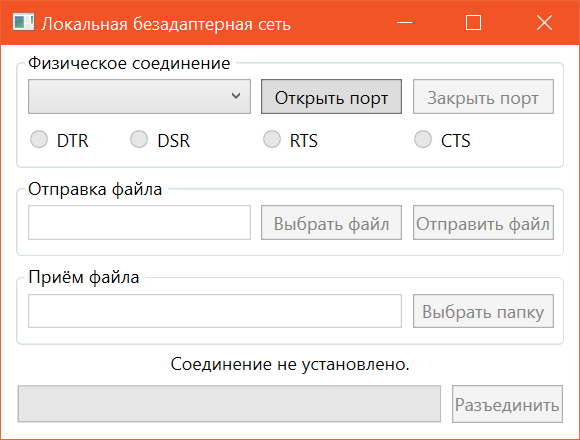
\includegraphics{window.png}
\caption{Главное окно программы.}\label{window}
\end{figure}
\begin{figure}
\centering
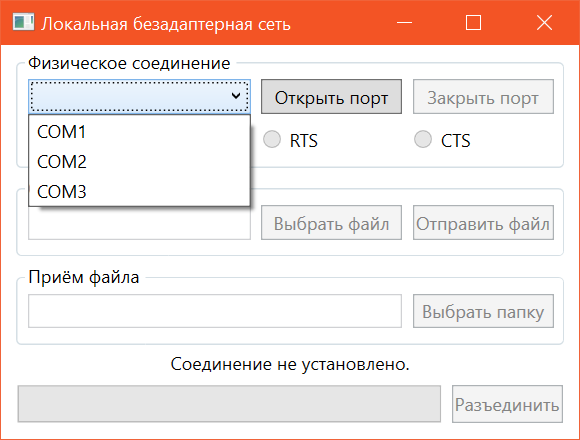
\includegraphics{list.png}
\caption{Выпадающий список доступных COM-портов.}\label{list}
\end{figure}
\begin{figure}
\centering
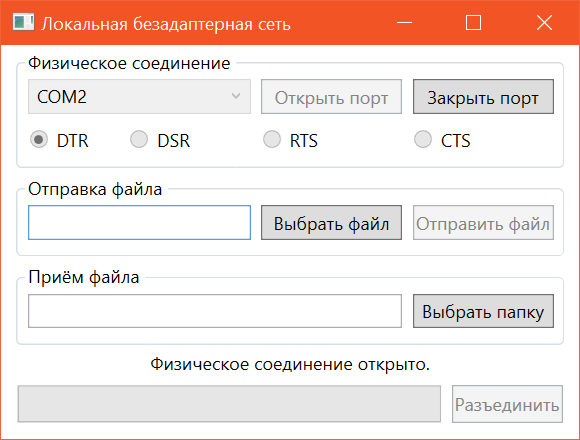
\includegraphics{open.png}
\caption{Окно программы после открытия физического соединения.}\label{open}
\end{figure}
\begin{figure}
\centering
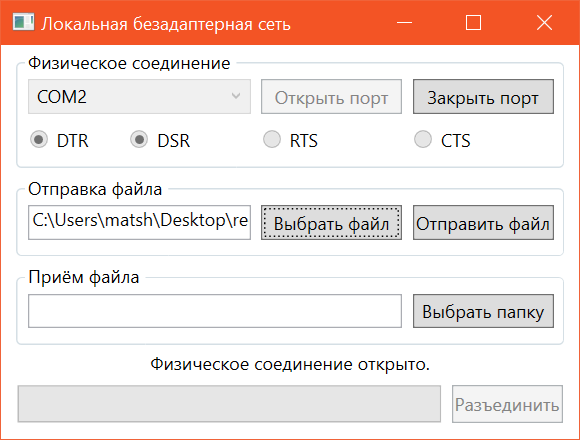
\includegraphics{send.png}
\caption{Окно программы после выбора файла.}\label{send}
\end{figure}
\begin{figure}
\centering
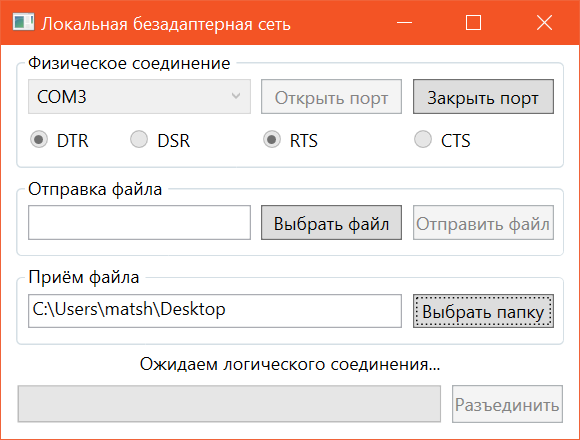
\includegraphics{select.png}
\caption{Окно программы после выбора папки.}\label{select}
\end{figure}
\begin{figure}
\centering
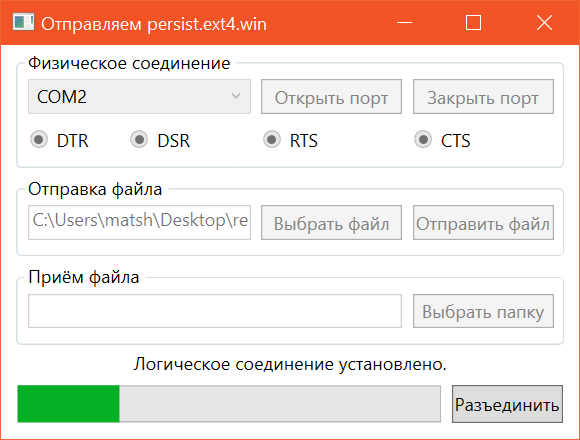
\includegraphics{progress.png}
\caption{Процесс передачи файла.}\label{progress}
\end{figure}
\begin{figure}
\centering
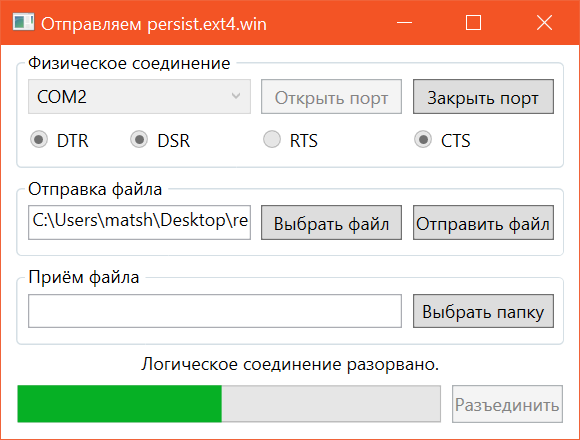
\includegraphics{disc.png}
\caption{Окно программы после принудительного разрыва соединения.}\label{disc}
\end{figure}
\begin{figure}
\centering
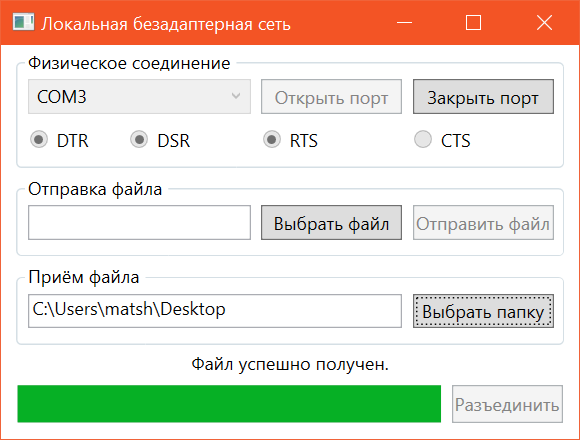
\includegraphics{fin.png}
\caption{Окно принимающей программы после приёма файла.}\label{fin}
\end{figure}

\end{document}